\chapter{Webots}
\label{sec:webots}


This documentation describes the \urbi engine for Webots.  Please go to
\url{http://www.gostai.com/doc/en/webots} to get the latest updated
version of this documentation.


% -------
% Chapter
% -------

\section{Quick Start}
\label{webots.quickstart}%

This section describes how to setup the software on your computer and
give you the basis to use \urbi for Webots.


\subsection{Setup}
\label{webots.setup}%

The setup process depends on your OS, please follow the corresponding
instructions.

Since different packages are available for Linux, you should use the
package which is designed for your distribution.

Warning: root privileges are required to install this software under
Linux.

\begin{table}[htbp]
  \begin{center}
    \begin{tabular}{p{.4\linewidth}l}
      \hline
      Linux distribution &    Package extension\\
      \hline
      RPM based distributions:
      \begin{itemize}
      \item CentOS
      \item Fedora Core
      \item Mandriva Linux
      \end{itemize}
      &
      rpm\\
      Debian based distributions
      \begin{itemize}
      \item Debian GNU/Linux
      \item Ubuntu
      \end{itemize}
      &
      deb \\
      Others
      \begin{itemize}
      \item Arch Linux
      \item Gentoo
      \item SUSE
      \end{itemize}
      &
      tarball (zip, tar.gz or tar.bz2)\\
      \hline
    \end{tabular}
  \end{center}
  \caption{Which package should I use?}
  \label{webots.setup.distributions}%
\end{table}

\subsubsection{Windows}
\label{webots.setup.windows}%

\paragraph{Installation}
\label{webots.setup.windows.installation}%

To install \urbi for Webots under windows, Webots must be installed on
your computer. If Webots is not installed, please first proceed to
Webots installation. Then double click on the ``\urbi Webots 1.0
Setup.exe'' and follow the instructions given by the installer:

\begin{enumerate}
\item The installer recommends to close all other running applications
  while installing \urbi for Webots. Click ``Next $>$'' to proceed.

\item Before installing \urbi for Webots, read and accept the Licence
  Agreement. Once you have read it, check ``I accept the agreement'' and
  click on ``Next $>$'' to proceed.

\item The installer will automatically detect your Webots installation
  path and install the \urbi controller, the worlds and data in the
  same location. For all the other files (\urbi for Webots SDK and
  \urbi for Webots Documentation) you have to provide a new
  location. This is what the installer is asking at this step. Choose
  a custom location if you don't want the default one,
  \nolinkurl{C:\Program Files\Gostai\\urbi Webots 1.0}, and click
  ``Next $>$'' to proceed.

\item In this step you can choose which features will be installed on
  your computer. Required features (``\urbi Webots'') cannot be
  unchecked. These are the \urbi controller and the Urbi for Webots
  worlds and data. They will be installed in your Webots installation
  directory. Optional features are the ``\urbi Software Development
  Kit'', useful if you want to develop your own UObjects and plug them
  in \urbi, and the ``\urbi Documentation''. Optional features will be
  installed in the location you provided at Step 3).  Check the
  checkbox near the features you want to install, and click ``Next $>$''
  to proceed to next step.

\item You can customize the location where shortcuts to \urbi files
  will be installed in you Start Menu. You can choose not to put any
  shortcuts just by checking ``Don't create a start menu folder''. Click
  ``Next $>$'' to proceed to next step.

\item \urbi source code files have a ``.u'' extension. By default the
  installer associate all ``.u'' files with \urbi. If you don't want
  these files to be associated unckeck the corresponding
  checkbox. Then click ``Next $>$'' to proceed to next step.

\item The installer prints a summary of the installation options for
  you to verify that it is correct. Then click ``Install'' to install
  \urbi for webots on your computer.

\item The installer display the README file. Click ``Next $>$'' to
  proceed to next step.

\item You have finished to install \urbi for Webots. Click ``Finish'' to
  close the installer.
\end{enumerate}

\subsubsection{Linux}
\label{webots.setup.linux}%

\paragraph{RPM based distributions}
\label{webots.setup.linux.rpm}%

Execute the following command:
\begin{shell}
$ rpm -hiv <package Urbi For Webots>.rpm
\end{shell}

\paragraph{Debian base distributions}
\label{webots.setup.linux.deb}%

Execute the following command:
\begin{shell}
$ sudo dpkg --install <package Urbi For Webots>.deb
\end{shell}%$

Your software is installed, you'll now have to setup the license.


\paragraph{Manual setup (from a tarball)}
\label{webots.setup.linux.tarball}%
as root

\begin{shell}
$ cd /
$ tar -xvzf  <package Urbi For Webots>.tgz
\end{shell}
or

\begin{shell}
$ cd /
$ tar -xvjf  <package Urbi For Webots>.tar.bz2
\end{shell}

\subsubsection{MacOs}
\label{webots.setup.macos}%

\paragraph{Manual install}
\label{webots.setup.macos.manual}%

You have to be administrator on your machine in order to install
UrbiForWebots.  Extract the zip file containing \urbi by double
clicking on it.  You obtain two folders: \nolinkurl{usr} and
\nolinkurl{webots}.  You have to copy the contains of the
\nolinkurl{webots} directory in the directory containing Webots
installation (if you did the default installation it is in
\nolinkurl{/Applications/Webots}), and you have to copy the contains
of the \nolinkurl{usr} folder in the \nolinkurl{/usr} system folder.


Let say you extracted the zip file in your \nolinkurl{Desktop} folder,
and that you set the variable WEBOTS\_HOME to the Webots installations
path as explained in Webots documentation.  From a shell terminal this
gives you:


\begin{shell}
$ cd $HOME/Desktop
$ ls
usr webots webots-urbiengine-sdk-webots-1.03-k1462-e247-l482-powerpc-apple-darwin8-gcc-4.0.1.zip
$ cp -r usr /
$ cp -r webots/* $WEBOTS_HOME/
\end{shell}

\subsection{Evaluation mode}
\label{webots.evaluation}%

If you don't provide a valid license file to the urbi controller, it
will be launched in evaluation mode. The only difference with the
normal version is that the controller will exit after 5 minutes, thus
letting you test all the feature we provide in the registered version
during this small period of time. When you launch Webots and \urbi
without a valid license file you can see a message in Webots log that
tells you that the license is invalid or missing:


%\begin{minipage}[c]{\linewidth}
%\begin{center}
%\imgexists{images/no-license-webots-log-msg.jpg}{{\centering \imgevalsize{images/no-license-webots-log-msg.jpg}{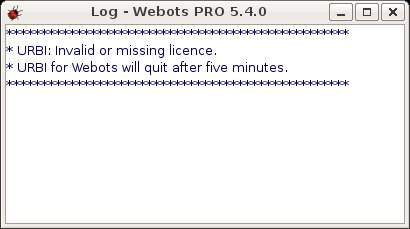
\includegraphics[width=\imgwidth,height=\imgheight,keepaspectratio=true]{images/no-license-webots-log-msg.jpg}}}}{}\end{center}
%\end{minipage}


\subsection{License setup}
\label{webots.license}%

In order to run Urbi for Webots unlimitedly you must have a licence
file .  The Urbi for Webots licensing system is based on the Webots
licensing system.  In Webots you have two licensing system available:
\begin{itemize}
\item a license file ``webots.key'';
\item an USB dongle;
\end{itemize}


\subsubsection{Urbi licensing with ``webots.key'' license}
\label{webots.license.webotskey}%

To obtain an Urbi license if you use this type of licensing, please
send us a copy of your webots.key license, we will generate the Urbi
license using this file.


Once you have your ``urbi.key'' file, put the ``webots.key'' file in the
folder:
\begin{itemize}

\item \nolinkurl{webots/ressources/}

\end{itemize}
(warning: it is mandatory to have a copy of the webots.key in this
folder, if you don't have it, Urbi won't find the webots.key file and
you will get a licensing error message) and place the ``urbi.key'' file
in the same folder as the urbi controller. By default in
\begin{itemize}

\item \nolinkurl{webots/projects/default/controllers/urbi/}

\end{itemize}


\subsubsection{Urbi licensing with USB dongle}
\label{webots.license.dongleusb}%

To obtain an Urbi license if you use this type of licensing, please
send us your Webots USB dongle number (available in the help/about
webots menu). We will then generate an Urbi license using this number.


Install your ``urbi.key'' file in the same folder as the Urbi
controller.  By default in
\begin{itemize}

\item  \nolinkurl{webots/projects/default/controllers/urbi/}

\end{itemize}


\subsection{License problem}
\label{webots.problem}%

If you have a valid license but still get the licensing error message,
verify that you have followed correctly the setup instructions. Note
that you can specify the location of the urbi.key license to the Urbi
controller, in the .wbt files, within the ``controllerArgs'' field. Just
add ``-{}l'' and the absolute path of your license file to the field
line. Exemple (with a license file urbi.key located in
\nolinkurl{C:/mylicensefolder/})

\begin{shell}
controllerArgs "-f -l C:/mylicensefolder/urbi.key  -p 54000 32 "
\end{shell}
Contact us at Gostai if you still have some problems with the license,
and we will resolve the problem with you.


\subsection{Your first run}
\label{webots.firstrun}%

This section describes basic use of the \urbi engine for Webots.


\subsubsection{\urbi worlds}
\label{webots.firstrun.openworld}%

We provide a set of example worlds with several robots you will be
able to control through \urbi. They are located in the directory:
\nolinkurl{WEBOTS_DIRECTORY/projects/packages/urbi/worlds/ }.  Open
the world named \nolinkurl{aibo_ers7_urbi_soccer.wbt}. The image
bellow is a screenshot of this world. You can see an aibo in a soccer
field, with a pink ball in front of it.


%\begin{minipage}[c]{\linewidth}
%\begin{center}
%\imgexists{images/webots-aibo-soccer.jpg}{{\centering \imgevalsize{images/webots-aibo-soccer.jpg}{\includegraphics[width=600pt,keepaspectratio=true]{images/webots-aibo-soccer.jpg}}}}{}\end{center}
%\end{minipage}


If you look in Webots scene tree, you will see that the aibo (real
name is ERS7) is a CustomRobot node, and that it uses urbi as
controller.


%\begin{minipage}[c]{\linewidth}
%\begin{center}
%\imgexists{images/webots-scene-tree.jpg}{{\centering \imgevalsize{images/webots-scene-tree.jpg}{\includegraphics[width=\imgwidth,height=\imgheight,keepaspectratio=true]{images/webots-scene-tree.jpg}}}}{}\end{center}
%\end{minipage}


Let's see how this controller let you control the robot.


\subsubsection{\urbi controller}
\label{webots.firstrun.urbicontroller}%

You have two ways to control your robot through the \urbi
controller. The first way is by remotely sending commands to the \urbi
controller. The \urbi controller act as a server, and let you connect
to it through the network, and then send \urbi commands to this server.
The second way is by writing \urbi scripts that will be loaded at
controller start up.


\subsubsection{Send commands with a client software}
\label{webots.firstrun.clientsoftware}%

In order to connect to the \urbi controller and then send commands, you
need to use a client software that allows you to connect on some
address on the network and let you send data through this connection.
The simplest program which do this is the \textbf{telnet} program,
available on all platform (Windows, Linux and MacOs). You can also use
one of the program available at Urbiforge (http://www.urbiforge.com)
in the Tool section.  The \urbi controller launched with the
aibo\_er7\_urbi\_soccer world is waiting for connections coming on
your computer, on port 54000. So to connect on it you will have to
specify the address of your computer ('localhost') and the right port
(54000).


\paragraph{Telnet}
\label{webots.firstrun.clientsoftware.telnet}%

\subparagraph{Windows}
\label{webots.firstrun.clientsoftware.telnet.windows}%

To launch \textbf{telnet} under windows click on the start menu, and
then on run.


%\begin{minipage}[c]{\linewidth}
%\begin{center}
%\imgexists{images/click-run-windows.gif}{{\centering \imgevalsize{images/click-run-windows.gif}{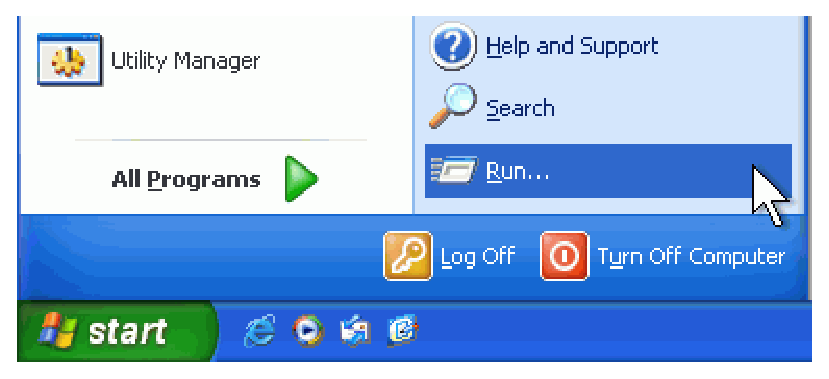
\includegraphics[width=\imgwidth,height=\imgheight,keepaspectratio=true]{images/click-run-windows.gif}}}}{}\end{center}
%\end{minipage}


Type \textbf{cmd} and click OK. This will launch a dos command prompt.


%\begin{minipage}[c]{\linewidth}
%\begin{center}
%\imgexists{images/run-cmd-windows.png}{{\centering \imgevalsize{images/run-cmd-windows.png}{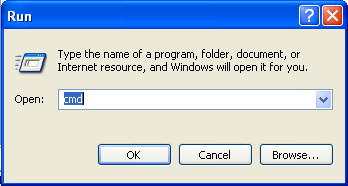
\includegraphics[width=\imgwidth,height=\imgheight,keepaspectratio=true]{images/run-cmd-windows.png}}}}{}\end{center}
%\end{minipage}


In the dos command prompt type \textbf{telnet localhost 54000}.


%\begin{minipage}[c]{\linewidth}
%\begin{center}
%\imgexists{images/telnet-windows.PNG}{{\centering \imgevalsize{images/telnet-windows.PNG}{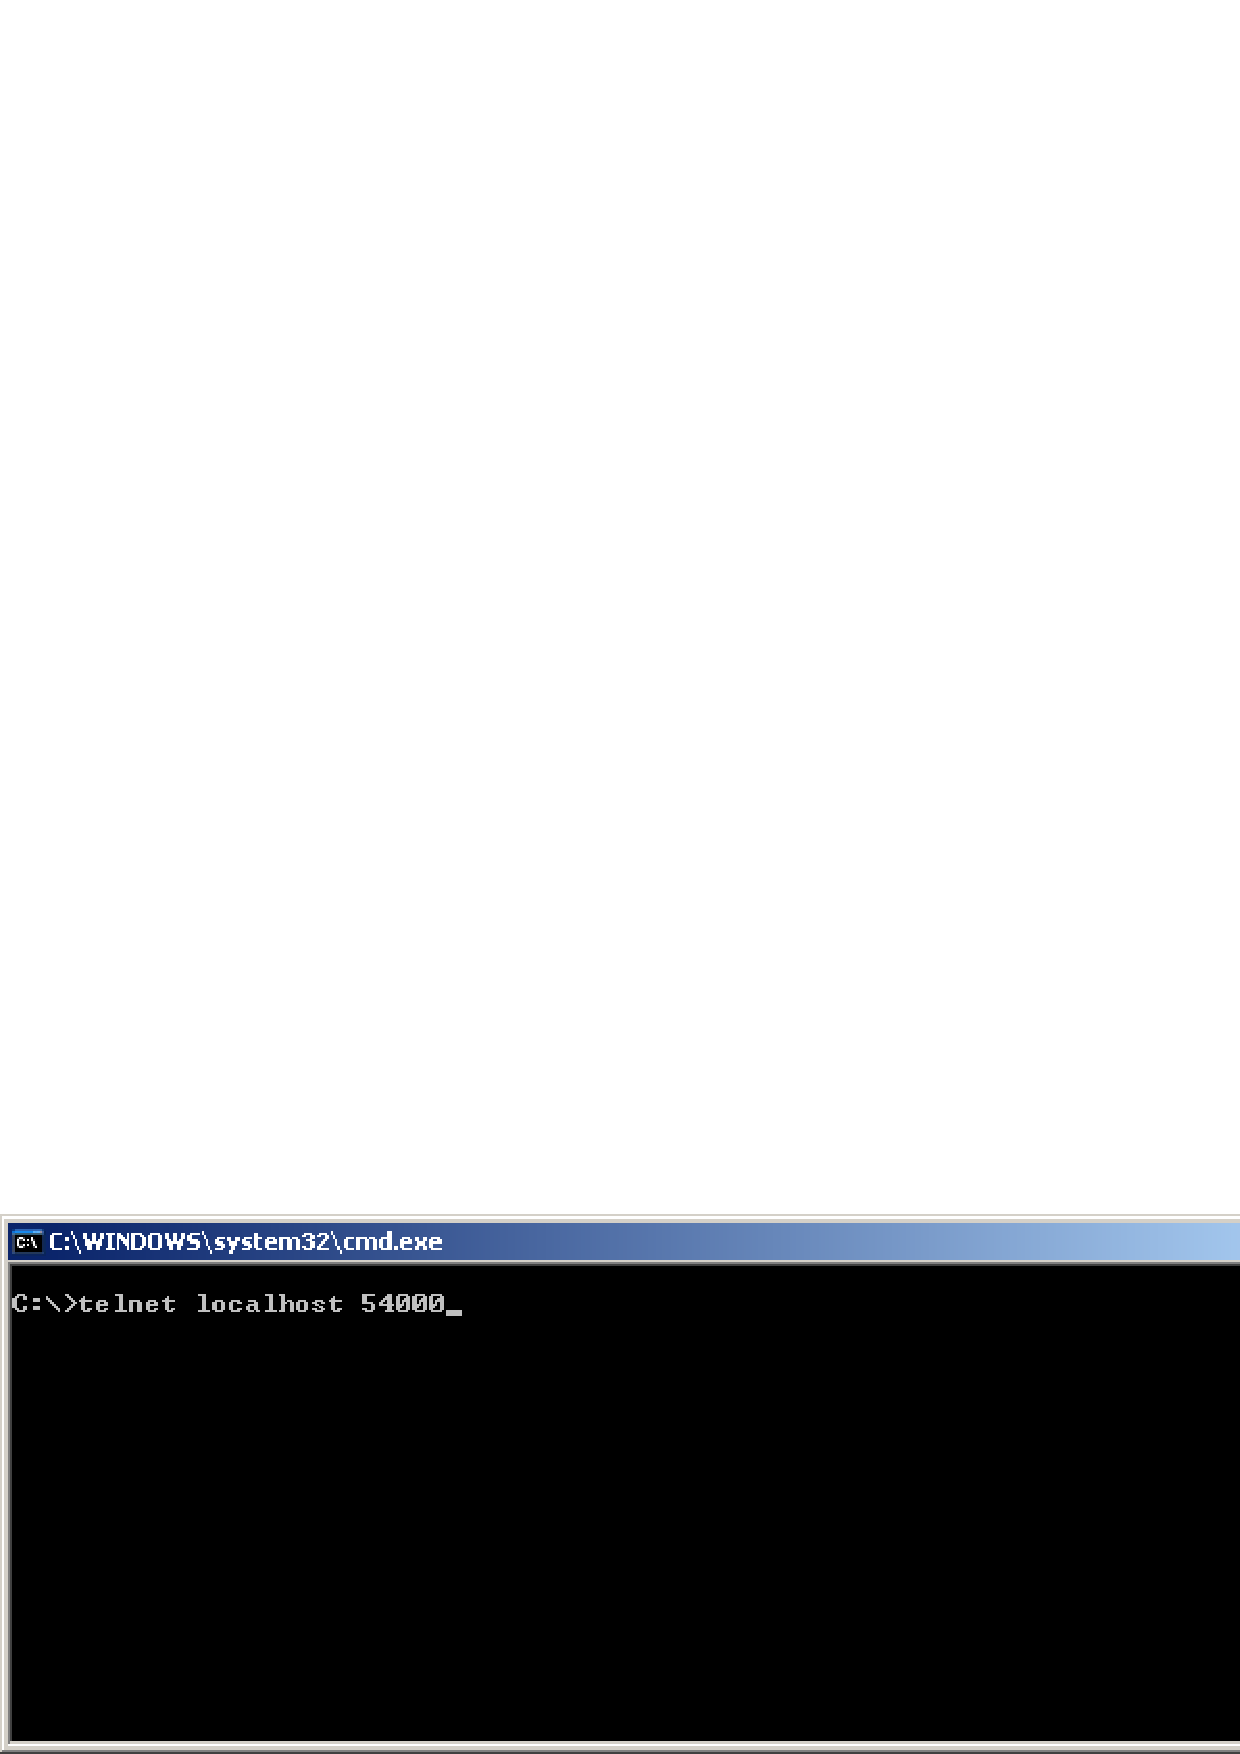
\includegraphics[width=\imgwidth,height=\imgheight,keepaspectratio=true]{images/telnet-windows.PNG}}}}{}\end{center}
%\end{minipage}


This launch telnet. It connect to the \urbi controller, and the \urbi
controller send you the \urbi header (the lines that display on the
screen). On windows the text is badly displayed because of some
character conversion problem. It is still usable even if it is not
really convenient.


%\begin{minipage}[c]{\linewidth}
%\begin{center}
%\imgexists{images/telnet-urbi-windows.PNG}{{\centering \imgevalsize{images/telnet-urbi-windows.PNG}{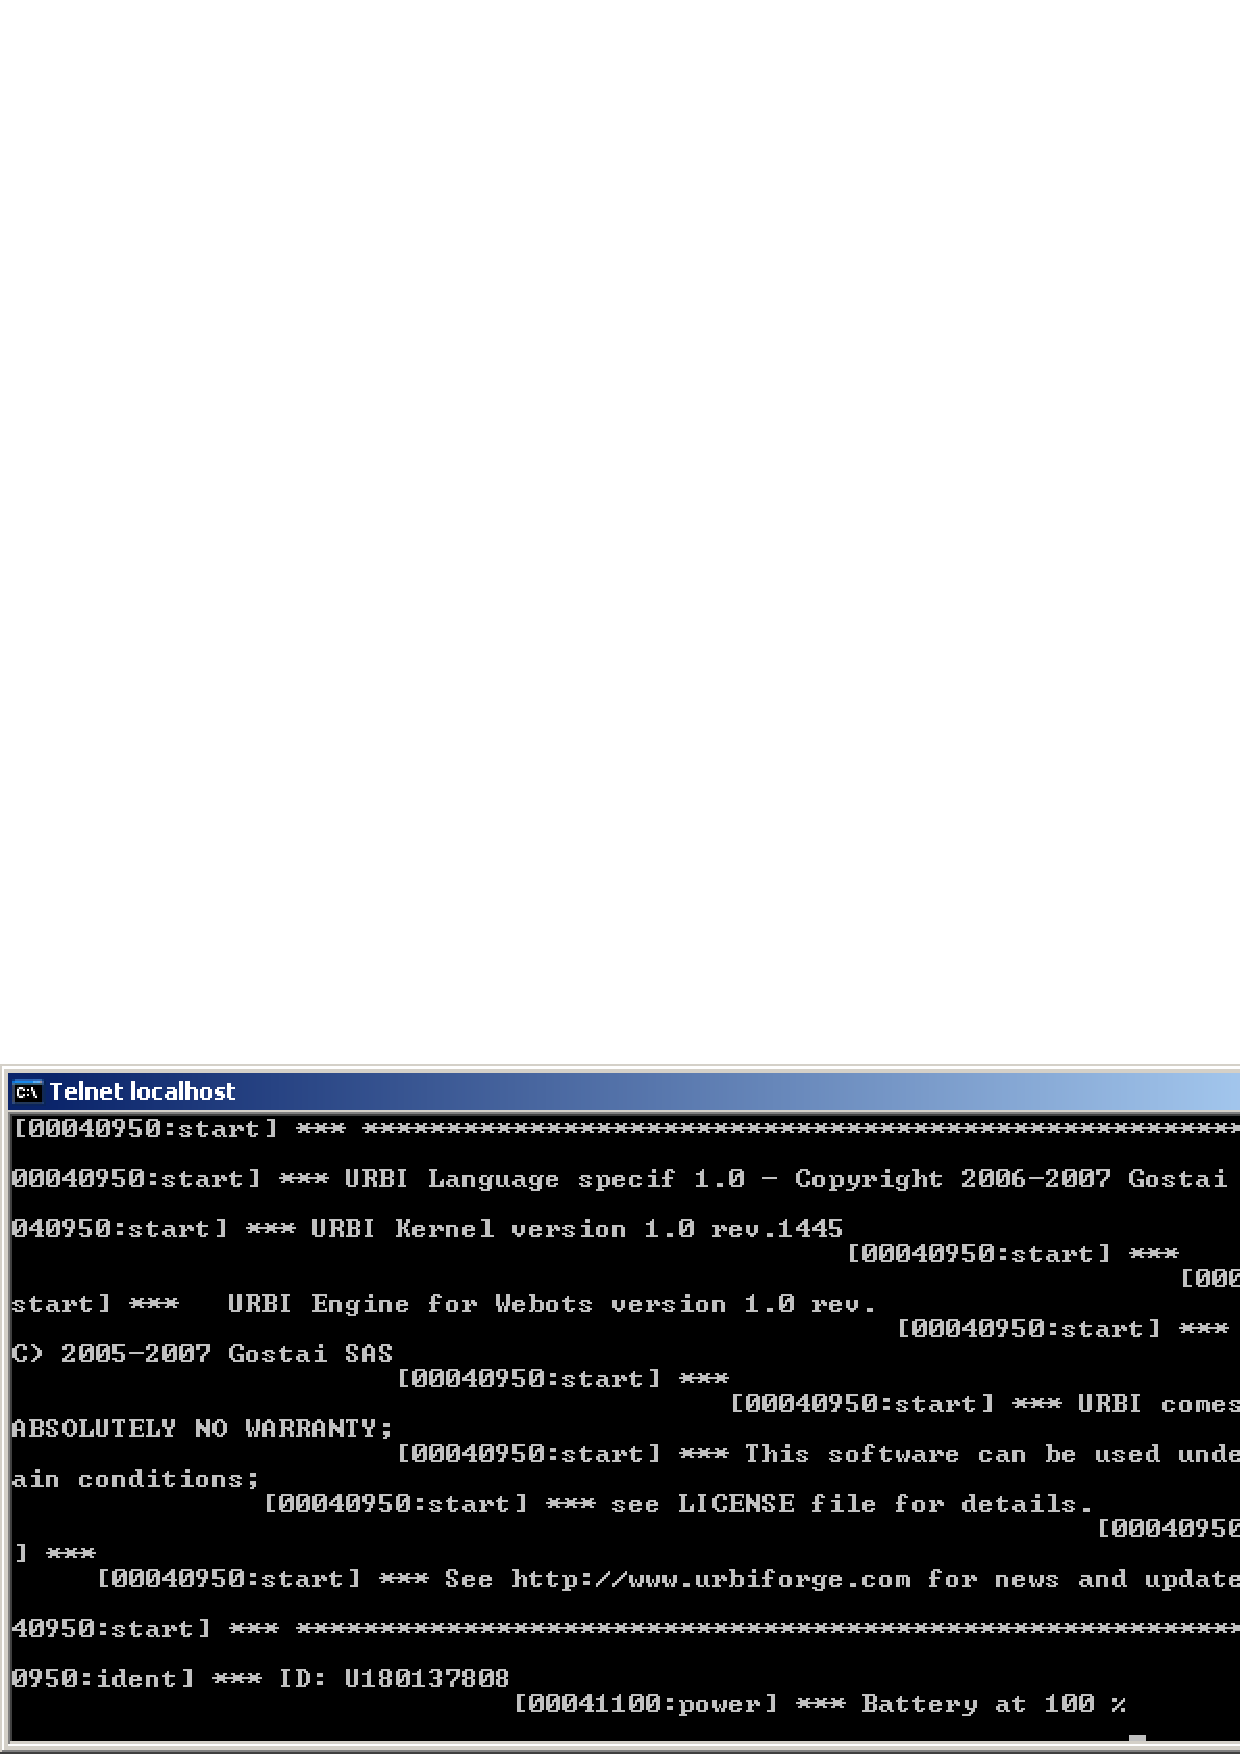
\includegraphics[width=\imgwidth,height=\imgheight,keepaspectratio=true]{images/telnet-urbi-windows.PNG}}}}{}\end{center}
%\end{minipage}


\subparagraph{Linux and MacOs}
\label{webots.firstrun.clientsoftware.telnet.linuxandmacos}%

Open a new shell and type \textbf{telnet localhost 54000}.  This
launch telnet. It connect to the \urbi controller, and the \urbi
controller send you the Urbi header.


%\begin{minipage}[c]{\linewidth}
%\begin{center}
%\imgexists{images/telnet-urbi-linux.jpg}{{\centering \imgevalsize{images/telnet-urbi-linux.jpg}{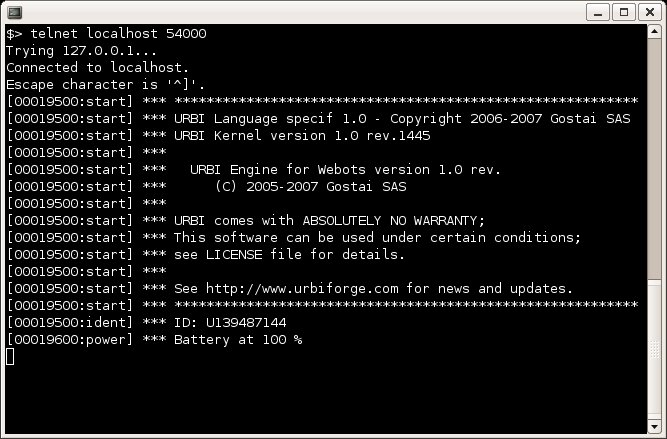
\includegraphics[width=\imgwidth,height=\imgheight,keepaspectratio=true]{images/telnet-urbi-linux.jpg}}}}{}\end{center}
%\end{minipage}


\subparagraph{Use telnet to send commands}
\label{webots.firstrun.clientsoftware.telnet.usetelnet}%

Now that you are connected to the \urbi controller, you can send
command to it and makes your robot move and interact with it's
environment. For example try typing the following commands in
\textbf{telnet}:

\begin{urbifixme}
headPan = 50 time: 5s;
headPan = -50 time: 5s;
headPan = 0 time: 5s;
\end{urbifixme}
And you will see the head of the aibo move left, right, and then to
the center.


%\begin{minipage}[c]{\linewidth}
%\begin{center}
%\imgexists{images/telnet-some-urbi-cmd.jpg}{{\centering \imgevalsize{images/telnet-some-urbi-cmd.jpg}{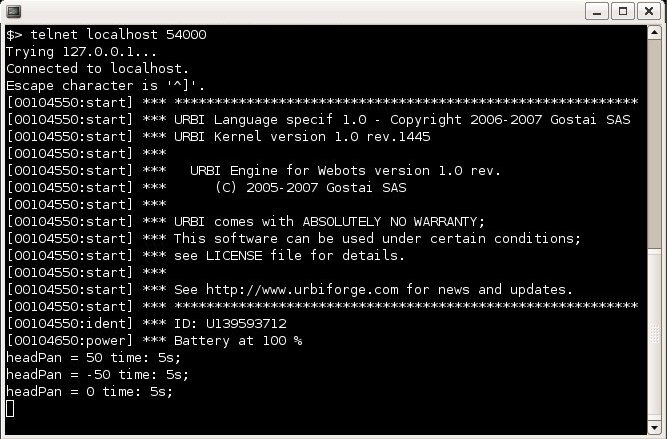
\includegraphics[width=\imgwidth,height=\imgheight,keepaspectratio=true]{images/telnet-some-urbi-cmd.jpg}}}}{}\end{center}
%\end{minipage}


\subsubsection{Load \urbi programs at controller start}
\label{webots.firstrun.loadprograms}%

\paragraph{By adding the file as argument of the \urbi controller}
\label{webots.firstrun.loadprograms.cmd_line}%

It is possible to write some \urbi script and load it at controller
startup.  To do this just write \urbi code in some file, and then
specify it's path in the controllerArgs webots node.  For example
create a new text file, rename it test.u and write in it:


\begin{urbifixme}
robot.sit (),
\end{urbifixme}

Then edit the webots world aibo\_ers7\_urbi\_soccer.wbt, and add the
path of your file test.u on the line of the controllerArgs node.


\begin{shell}
controllerArgs "-f -p 54000 32 [HERE ADD YOUR SCRIPT FILES]"
\end{shell}

For exemple let say that you created your file in
\begin{itemize}

\item C:/Program Files/webots/projects/packages/urbi/data/aibo/ (under
  Windows)



\item /Applications/webots/projects/packages/urbi/data/aibo/ (under
  Macos)



\item /usr/local/webots/projects/packages/urbi/data/aibo/ (under
  Linux)


\end{itemize}
        Then you can specify the path to your file in a absolute form:
 \begin{itemize}

\item   C:/Program Files/webots/projects/packages/urbi/data/aibo/test.u (under Windows)



\item   /Applications/webots/projects/packages/urbi/data/aibo/test.u (under Macos)



\item   /usr/local/webots/projects/packages/urbi/data/aibo/test.u (under Linux)


\end{itemize}
       Or you can specify it's path relativelly to the Urbi controller location.
      Let say that you are using the Urbi controller located here:
 \begin{itemize}

\item   C:/Program Files/webots/projects/default/controllers/urbi/urbi (under Windows)



\item   /Applications/webots/projects/default/controllers/urbi/urbi (under Macos)



\item   /usr/local/webots/projects/default/controllers/urbi/urbi (under Linux).


\end{itemize}
       Then the path to your file relatively to the Urbi controller is:
 \begin{itemize}

\item   ../../../packages/urbi/data/aibo/test.u (under Windows|Linux|Macos)


\end{itemize}
         Add this path to the controllerArgs line and it gives:


\begin{shell}
# Under Windows, absolute path version:
controllerArgs "-f -p 54000 50 \"C:/Program Files/webots/projects/packages/urbi/data/aibo/test.u\""
(note the use of \" \" about the path, which are mandatory if the path
contains spaces. Here between Program and Files)

# Under MacOs, absolute path version:
controllerArgs "-f -p 54000 50 /Applications/webots/projects/packages/urbi/data/aibo/test.u"

# Under Linux, absolute path version:
controllerArgs "-f -p 54000 50 /usr/local/webots/projects/packages/urbi/data/aibo/test.u"

# Relative path version (os independant)
controllerArgs "-f -p 54000 50 ../../../packages/urbi/data/aibo/test.u"
\end{shell}

NB: If you have some spaces in your file path, you have to add
backslashed double quotes in order to have webots and Urbi understand
the path correctly.


Now when you launch Webots and you open the world
aibo\_ers7\_urbi\_soccer.wbt you can verify that the controllerArgs
was correctly updated.


%\begin{minipage}[c]{\linewidth}
%\begin{center}
%\imgexists{images/webots-scene-tree-add-loaded-file.jpg}{{\centering \imgevalsize{images/webots-scene-tree-add-loaded-file.jpg}{\includegraphics[width=\imgwidth,height=\imgheight,keepaspectratio=true]{images/webots-scene-tree-add-loaded-file.jpg}}}}{}\end{center}
%\end{minipage}


And if you look at the world view, you can see that the controller has
executed the \urbi code you specified: the aibo has sat.


%\begin{minipage}[c]{\linewidth}
%\begin{center}
%\imgexists{images/webots-aibo-sat.jpg}{{\centering \imgevalsize{images/webots-aibo-sat.jpg}{\includegraphics[width=400pt,keepaspectratio=true]{images/webots-aibo-sat.jpg}}}}{}\end{center}
%\end{minipage}


\paragraph{By loading the file in \urbi.ini}
\label{webots.firstrun.loadprograms.inurbiinifile}

By default, we don't specify files on the Webots controllerArg
line. We specify directories.  At startup, the \urbi controller will go
through these directories and try to find a file named
\nolinkurl{\urbi.ini}. This is a special file containing \urbi code
which is always loaded at start up by the \urbi controller. So another
way to load your custom \urbi code at start up is to use the command
'load'.  Take the \nolinkurl{test.u} file we created in the previous
section and move it to the folder containing the \nolinkurl{\urbi.ini}
file. Then open \nolinkurl{\urbi.ini} and add at the end of the file:


\begin{urbifixme}
load ("test.u");
\end{urbifixme}
Now launch Webots and open the world using the \urbi controller loading
the \urbi.ini you just updated, and you will see that your code has
been loaded too.

% -------
% Chapter
% -------

\section{Built-{}in robots and worlds}
\label{webots.builtin}%

This section deals with the robots and worlds provided with the the
engine.


\subsection{Understanding the \urbi for Webots hierarchy}
\label{webots.builtin.hierarchy}%

 Urbi for Webots is bundled with a lot of files. Here is a description of
those files.

\begin{table}[htbp]
\begin{center}
\begin{tabular}{ll}\hline
  Directory &   Description \\
  webots/projects/default/controllers & Contains the \urbi controller. \\
  webots/projects/default/controllers/urbi &      \\
  webots/projects/default/controllers/urbi/urbi &       Controller's binary \\
  webots/projects/default/controllers/urbi/urbi.key &   \urbi for Webots license key \\
  webots/resources/webots.key & Webots license key \\
  webots/projects/packages/urbi/data &  Data directory (\urbi scripts and misc. multimedia files) \\
  webots/projects/packages/urbi/data/aibo &     Main Aibo robots directory \\
  webots/projects/packages/urbi/data/aibo/ers7 &        Aibo ERS-7 directory \\
  webots/projects/packages/urbi/data/aibo/ers210 &      Aibo ERS-210 directory \\
  webots/projects/packages/urbi/data/aibo/ers210 &      Aibo ERS-220 directory \\
  webots/projects/packages/urbi/data/e-puck &   E-puck robots directory \\
  webots/projects/packages/urbi/data/kiki &     Kiki robots directory \\
  webots/projects/packages/urbi/data/pioneer2 & Pioneer2 robots directory \\
  webots/projects/packages/urbi/data/ustd &     Ustd directory (please see Ustd dedicated documentation for more information) \\
  webots/projects/packages/urbi/worlds &        \urbi for Webots worlds directory \\
  webots/projects/packages/urbi/worlds/aibo\_ers210\_urbi.wbt & Main world for the Aibo ERS-210. \\
  webots/projects/packages/urbi/worlds/aibo\_ers7\_urbi.wbt &   Main world for the Aibo ERS-7. \\
  webots/projects/packages/urbi/worlds/aibo\_ers7\_urbi\_soccer.wbt &   Soccer world for the Aibo ERS-7. \\
  webots/projects/packages/urbi/worlds/aibo\_ers7\_urbi\_supervisor.wbt &       Supervisor world for the Aibo ERS-7 (see the supervisor section). \\
  webots/projects/packages/urbi/worlds/e-puck\_urbi.wbt &       Main world for the e-puck. \\
  webots/projects/packages/urbi/worlds/kiki\_urbi.wbt & Main world for the kiki example robot. \\
  webots/projects/packages/urbi/worlds/pioneer2\_urbi.wbt &     Main world for the Pioneer 2. \\
  webots/projects/packages/urbi/worlds/textures &       World's textures directory. \\
\hline
\end{tabular}
\end{center}

\caption{Directory hierarchy}
\label{webots.builtin.directory}%
\end{table}

 It is important to notice the data's directory hierarchy, each path follows
the following rule:


\begin{lstlisting}
data/<ROBOT NAME>
\end{lstlisting}

If several version of the robots are available, the following
rule is applied:

\begin{lstlisting}
data/<ROBOT NAME>/<VERSION>
\end{lstlisting}

 In those directories, standard files are:

\begin{table}[htbp]
\begin{center}
\begin{tabular}{ll}\hline
  File &        Description \\
  CLIENT.INI &  Client initialization script (required). \\
  config.u &    Configuration file (used to customize the robot). \\
  <ROBOT>.ini & Robot hardware layout. \\
  \urbi.INI &    Server initialization script (required). \\
\hline
\end{tabular}
\end{center}

\caption{Standard robot's files}
\label{webots.builtin.files}%
\end{table}

\subsection{Worlds special features}
\label{webots.builtin.worlds}%

 This section describes the special features of some worlds.
The worlds referenced in the previous section as the ``main''
world have no specificities.


\subsubsection{The soccer world (balltracking)}
\label{webots.builtin.worlds.soccer}%

 Launch Webots and load the soccer world
(\nolinkurl{aibo_ers7_urbi_soccer.wbt}).


Connect to the \urbi server and use the following command:

\begin{urbifixme}
unfreeze balltracking;
\end{urbifixme}

 This will activate the balltracking of the ERS-{}7 robot.
Now, you can use \textbf{shift} and the mouse to move
the ball, the ERS-{}7 will move its head to follow the ball.


\subsubsection{The supervisor world}
\label{webots.builtin.worlds.supervisor}%

 Launch Webots and load the supervisor world
(\nolinkurl{aibo_ers7_urbi_supervisor.wbt}).


 It is crucial to understand that this world launches two \urbi servers.
The robot's server on the port 54001 and the supervisor server on the
port 54002.


 A supervisor is a kind of robot in Webots which can be used ton control
the world. It is used, for example, in the Webots soccer example to give
the ball's position.


 If you create a supervisor node which is linked to an \urbi controller,
this will allow you to control the world through \urbi.


 Warning: don't forget to give different ports for each robot you add in a
Webots world. If this is not the case, some controllers will not work.


 After having started the simulation of the supervisor world, execute
the following lines:


\begin{urbifixme}
// Create a moving label.
l = new Label("\urbi for Webots");
l.size = 0.04;
l.r = 125 sin:10s ampli:125,
l.x = 0.2 sin:10s ampli:0.1,

// Manipulate the floor.
fl = new ManipulateNode("FLOOR");
fl.ty = -1 sin:10s ampli:0.5,
\end{urbifixme}

 The first part of the script creates a label and defines a movement
with the sin modifier. The second part moves the floor.


For a complete documentation of those nodes, please read the
next sections.

\subsection{Robots specific functions}
\label{webots.builtin.robots}%

 A lot of functions are directly available in \urbi to generate
high-{}level behaviour. Those features will be described in the
next section.


\subsubsection{Aibo specific functions}
\label{webots.builtin.robots.aibo}%

 The following table sums up the aibo's functions.

\begin{itemize}
\item \lstinline|robot.walk(duration)|\\
  Walk for duration milliseconds (walk backward if duration is negative).
\item \lstinline|robot.stopwalk()|\\
  Interrupt the walk.
\item \lstinline|robot.turn(duration)|\\
  Turn counter-clockwise for duration milliseconds (turn backward if duration is negative).
\item \lstinline|robot.stopturn()|\\
  Interrupt the turn.
\item \lstinline|robot.initial()|\\
  Initial position sitting down (stretch and lay).
\item \lstinline|robot.stretch()|\\
  Stretching like in the morning...
\item \lstinline|robot.lay()|\\
  Laying (sitting down).
\item \lstinline|robot.sit()|\\
  Sit on the back.
\item \lstinline|robot.beg()|\\
  Stand up with knees bent.
\item \lstinline|robot.stand()|\\
  Stand up.
\end{itemize}

\begin{itemize}
\item \lstinline|robot.walkspeed|\\
  speed of walk, the smaller the faster: period of a step. Defaults to
  1s.
\item \lstinline|robot.turnspeed|\\
  Speed of turn, the smaller the faster: period of a step. Defaults to
  1s.
\end{itemize}

More high-level behaviours are available in \nolinkurl{ustd}, please
read the corresponding documentation to obtain more information.


% -------
% Chapter
% -------

\section{Making your own \urbi for Webots controllers}
\label{webots.own}%

\subsection{Create from an existing world}
\label{webots.own.create}%

     As soon as you will want to go further, you will have to create your own
    \urbi for Webots based controllers. Here is how to proceed:

\begin{enumerate}

\item      Create a new directory in your \nolinkurl{data} directory
     (say \nolinkurl{foo}). This directory should be named as your
     new robot.



\item      Copy into your \nolinkurl{foo} directory the content
     of the kiki directory.



\item     Edit the \nolinkurl{kiki.ini} file and rename it into your
    robot's name (i.e. \nolinkurl{foo.ini} in this example).



\item     Edit the \nolinkurl{\urbi.INI} file and change the line:


\begin{urbifixme}
load("kiki.ini");
\end{urbifixme}

by:

\begin{urbifixme}
load("foo.ini"); // The name should match with the file you've just renamed.
\end{urbifixme}




\item Copy the kiki world file (\nolinkurl{worlds/kiki_urbi.wbt}
  should be copied into \nolinkurl{worlds/foo_urbi.wbt} for example).


  Edit your new world file and check that the field ControllerArgs
  contains the directory you've just created. It should be, for
  example: \texttt{-{}\-p 5\-4\-0\-0\-0 5\-0
    .\-.\-/\-.\-.\-/\-.\-.\-/\-p\-a\-c\-k\-a\-g\-e\-s\-/\-u\-r\-b\-i\-/\-d\-a\-t\-a\-/\-f\-o\-o}.
  The Controller field should keep its value to \texttt{u\-r\-b\-i}.


\end{enumerate}

Your robot is now ready to be controlled by \urbi. During the next
part, you'll learn how to customize the robot you have created.


\subsection{Customize}
\label{webots.own.customize}%

To handle each robots' specificities, Webots use a set of devices
which is fully supported by \urbi for Webots. Those devices are created
in a special file which is called like your robot in its data
directory. With the previous example, it would have been the
\nolinkurl{data/foo/foo.ini} file. This file should be like the
following piece of code:


\begin{urbifixme}
system.name = "/gostai/webots/kiki";
system.type = "webots";


wheelL = new DifferentialWheels("kiki", true);
alias wheelL.val wheelL.speed;
wheelR = new DifferentialWheels("kiki", false);
group wheels {wheelL, wheelR};

alias wheelR.val wheelR.speed;
eyeL = new DistanceSensor("ir0");
eyeR = new DistanceSensor("ir1");

// Standard groups
group software {};
group hardware {wheelL, wheelR, eyeL, eyeR};
group objects {software, hardware};

// Standard aliases
// etc.
\end{urbifixme}

The first line is your robot's name, you may edit this to any value.
The second line must keep its value.


After this, you need to create your robot's devices. It's very easy:
you just have to follow the rule: \texttt{
  d\-e\-v\-i\-c\-e\-n\-a\-m\-e = n\-e\-w
  d\-e\-v\-i\-c\-e\-t\-y\-p\-e\-(\-"\-n\-a\-m\-e o\-f t\-h\-e
  d\-e\-v\-i\-c\-e\-'\-s n\-o\-d\-e i\-n t\-h\-e w\-o\-r\-l\-d
  f\-i\-l\-e\-"\-)\-;\- }

The node name can be retrieved easily from the Webots world tree
editor.

One exception is the
\texttt{D\-i\-f\-f\-e\-r\-e\-n\-t\-i\-a\-l\-W\-h\-e\-e\-l} device.
There is always two lines. The first has its second argument set to
\texttt{t\-r\-u\-e} and will create the left wheel. The second with
its second argument set to \texttt{f\-a\-l\-s\-e} create the right
wheel.


The last step is editing the groups to add your new devices. The
hardware group should contain all the devices your robot uses. You may
also create subgroup to ease robot's programming.


\subsection{Urbi controller options}
\label{webots.own.controlleroptions}%

 The Urbi controller can take several options which modify it's behaviour.
You specify the controller options in the controllerArgs field of the Webots
world (.wbt) files.
 The controllerArgs must be as follow:

\begin{shell}
controllerArgs [options] period [path1 path2 ...]
\end{shell}
\begin{itemize}

\item period: base \urbi interval in milliseconds. You have to set the
  same period for the Urbi controller and for the Webots worlds. The
  period in the webots world is defined in the field ``basicTimeStep''.


\item [path ..] items are absolute or relative path elements searched
  in order to find Urbi files when 'load' is called.


\item options:
  \begin{itemize}

  \item -{}f : enable fast mode: the server will run as fast as
    possible and emulate the period specified.  Don't set -{}f option
    when there is ``runRealTime TRUE'' in the Webots world.  Always set
    -{}f otherwise.


  \item -{}l license\_key : specify the license key to use


  \item -{}p port : specify the tcp port \urbi will listen to.

  \end{itemize}

\end{itemize}


% -------
% Chapter
% -------

\section{Available UObjects}
\label{webots.uobjects}%

\subsection{Robot devices UObjects}
\label{webots.uobjects.robotdevices}%

\subsubsection{Accelerometer}
\label{webots.uobjects.robotdevices.accelerometer}%

\paragraph{Constructor}
\label{webots.uobjects.robotdevices.accelerometer.constructor}%

\noindent
\begin{description}
\item[{Accelerometer (string NodeName, string ComponentName)}]
  Construct a new Accelerometer object.  The ``NodeName'' attribute is
  the value of the name field, in the Accelerometer node in Webots.
  The ``ComponentName'' is the name of the Accelerometer component this
  object represent.  Because you need 3 Accelerometer UObject to
  represent the Webots Accelerometer device. Each Accelerometer
  UObject represent one of the component of the Webots Accelerometer
  device.  ``ComponentName'' can take 3 values: ``x'', ``y'' or ``z''.

\end{description}

\paragraph{Attributes}
\label{webots.uobjects.robotdevices.accelerometer.attributes}%

\noindent
\begin{description}
\item[{load}] Permissions: readable, writeable.


  Type: float.


  Range: \{0,1\}


  Description: This attribute let you enable or disable the
  Accelerometer device.  By default it is set to 1, which means that
  the Accelerometer is enabled. If you set it to 0 it will disable
  it. NB: If you enable or disable one of the Accelerometer UObject
  component, then all the associated Accelerometer UObject components
  will also be enabled or disabled (ex: if you disable the y
  Accelerometer component, then the x and z Accelerometer components
  will also be disabled).


  To enable and disable the device we use the following Webots
  functions:


\begin{lstlisting}
  void accelerometer_enable (DeviceTag sensor, unsigned short ms);
  void accelerometer_disable (DeviceTag sensor);
\end{lstlisting}

The frequency given to the enable function is the frequency of the
\urbi controller (given in the ``controllerArgs'' field in the .wbt
file).

\item[{ val }] Permissions: readable.


  Type: float.


  Description: The value of the component this UObject represent. So
  it is one of the 3 component of the Webots Accelerometer
  device. Either x, y or z.


  Retrieved with the following Webots functions:


\begin{lstlisting}
  const float *accelerometer_get_values (DeviceTag sensor); float
  accelerometer_value_x (float *array); float accelerometer_value_y
  (float *array); float accelerometer_value_z (float *array);
\end{lstlisting}
\end{description}

\subsubsection{Camera}
\label{webots.uobjects.robotdevices.camera}%

   The camera UObject lets you control a Webots camera device. When your robot
  possess a camera, and it use
  \urbi as a controller, you won't see the camera image displayed on your computer
  screen unless you create this camera UObject. You can create only one
  camera Urbi Object by Webots camera device. Once you have created the camera,
  the camera image will be displayed in the place defined by the .wbt world.


\paragraph{Constructor}
\label{webots.uobjects.robotdevices.camera.constructor}%

\noindent
\begin{description}
\item[{Camera (string NodeName)}] Construct a new camera object. The ``NodeName'' attribute is the value
          of the name field, in the camera node in Webots.

\end{description}

\paragraph{Attributes}
\label{webots.uobjects.robotdevices.camera.attributes}%

\noindent
\begin{description}
\item[{load}] Permissions: readable, writeable.


  Type: float.


  Range: \{0,1\}


  Description: This attribute let you enable or disable the camera
  device.  By default it is set to 1, which means that the camera is
  enabled. If you set it to 0 it will disable it.  To enable and
  disable the device we use the following Webots functions:


\begin{lstlisting}
  void camera_enable (DeviceTag camera, unsigned short ms); void
  camera_disable (DeviceTag camera);
\end{lstlisting}

The frequency given to the enable function is the frequency of the
\urbi controller (given in the ``controllerArgs'' field in the .wbt
file).

\item[{val}] Permissions: readable.


  Type: binary.


  Description:The current image acquired by the camera. The format of
  the image can be RGB, JPEG or YCbCr, and is determined by the
  ``format'' attribute.  To retrieve the camera image we use the
  following Webots function:


\begin{lstlisting}
  unsigned char *camera_get_image (DeviceTag camera);
\end{lstlisting}
\item[{format}] Permissions: readable, writable.


  Type: float.


  Range: \{0,1,2\}


  Description: The format of the camera image for the ``val''
  attribute. Set format to:

  \begin{description}
  \item[0] for JPEG;
  \item[1] for YCbCr;
  \item[2] for RGB;
  \end{description}

\item[{rgb}] Permissions: readable.


  Type: binary.


  Description: The current image acquired by the camera with format
  RGB.

\item[{jpeg}] Permissions: readable.


  Type: binary.


  Description: The current image acquired by the camera with format
  JPEG.

\item[{ycbcr}] Permissions: readable.


  Type: binary.


  Description: The current image acquired by the camera with format
  YCbCr.

\item[{jpegfactor}] Permissions: readable, writeable.


  Type: float.


  Range: [0;100]


  Description: Compression factor in JPEG mode.
\item[{width}] Permissions: readable.


  Type: float.


  Description: Image width. Retrieved with the following Webots
  function:


\begin{lstlisting}
  unsigned short camera_get_width (DeviceTag camera);
\end{lstlisting}
\item[{height}] Permissions: readable.


  Type: float.


  Description: Image height. Retrieved with the following Webots
  function:


\begin{lstlisting}
  unsigned short camera_get_height (DeviceTag camera);
\end{lstlisting}
\item[{xfov}] Permissions: readable, writeable.


  Type: float.


  Description: Image horizontal focal view.  Retrieved and set with
  the following Webots function:


\begin{lstlisting}
  float camera_get_fov (DeviceTag camera); void camera_set_fov
  (DeviceTag camera, float fov);
\end{lstlisting}
\item[{yfov}] Permissions: readable, writeable.


  Type: float.


  Description: Image vertical focal view. Calculated from the value of
  the horizontal focal view with the formula: yfov = xfov * height /
  width.

\item[{near}] Permissions: readable.


  Type: float.


  Description: Distance of the camera to the near OpenGL clipping
  plane.  Retrieved with the following Webots function:


\begin{lstlisting}
  float camera_get_near (DeviceTag camera);
\end{lstlisting}
\item[{far}] Permissions: readable.


  Type: float.


  Description: Distance of the camera to the far OpenGL clipping
  plane.  Retrieved with the following Webots function:


\begin{lstlisting}
  float camera_get_far (DeviceTag camera);
\end{lstlisting}
\end{description}

\subsubsection{Differential Wheels}
\label{webots.uobjects.robotdevices.differentialwheels}%

\paragraph{Constructor}
\label{webots.uobjects.robotdevices.differentialwheels.constructor}%

\noindent
\begin{description}
\item[{DifferentialWheels (string NodeName, boolean isLeft)}]
  Construct a new differential wheels object. You have to set true or
  false in the isLeft field to set whether the wheel you are
  constructing is the left or right wheel.  NB: DifferentialWheels
  goes by pair, so you must create the two DifferentialWheels objects
  for them to behave correctly.

  Example:

\begin{lstlisting}
  wheelL = new DifferentialWheels("e-puck", true); wheelR = new
  DifferentialWheels("e-puck", false);
\end{lstlisting}
\end{description}

\paragraph{Attributes}
\label{webots.uobjects.robotdevices.differentialwheels.attributes}%

\noindent
\begin{description}
\item[{encoder}] Permissions: readable, writeable.


  Type: float.


  Definition: Encoders are counters incremented each time a wheel
  turns. The amount added to the encoder is computed from the angle
  the wheel have been rotated and from the ``encoderResolution''
  parameter of the DifferentialWheels node. For convenience we also
  provide an ``encoderFactor'' which allows you to change easily the
  unit of the encoder on the Urbi side.  Hence, if the
  ``encoderResolution'' is 100, the ``encoderFactor'' is -{}1 and the
  wheel made a whole revolution, the corresponding encoder will have
  its value incremented by about 100 * -{}1 * 6.28 = -{}628.  Setting
  encoders value will not make the wheels rotate to reach the
  specified value, instead, it will simply reset the encoders with the
  specified value.  Retrieved and set with the following Webots
  functions:


\begin{lstlisting}
  int differential_wheels_get_left_encoder (void); int
  differential_wheels_get_right_encoder (void); void
  differential_wheels_set_encoders (int left, int right);
\end{lstlisting}
\item[{speed}] Permissions: readable, writeable.


  Type: float.


  Definition: Current speed of the wheels. The speed unit is defined
  by the ``speedUnit'' field of the Webots DifferentialWheels node. The
  default value is 0.1 radian per seconds. For convenience we also
  provide an ``speedFactor'' which allows you to change easily the unit
  of the speed on the Urbi side.  With a ``speedFactor'' of 10, a speed
  value of 20 will make the wheel rotate at a speed of 10 * 20 * 0.1 =
  20 radian per seconds.  Set with the following Webots function:


\begin{lstlisting}
  void differential_wheels_set_speed(short left, short right);
\end{lstlisting}
\item[{speedFactor}] Permissions: readable, writeable.


  Type: float.


  Definition: Convenient variable to set the speed unit. See ``speed''
  attribute.

\item[{encoderFactor}] Permissions: readable, writeable.


  Type: float.


  Definition: Convenient variable to set the encoder unit. See
  ``encoder'' attribute

\end{description}

\subsubsection{Distance Sensor}
\label{webots.uobjects.robotdevices.distancesensor}%

\paragraph{Constructor}
\label{webots.uobjects.robotdevices.distancesensor.constructor}%

\noindent
\begin{description}
\item[{DistanceSensor (string NodeName)}]         Construct a new Distance Sensor object, corresponding to the DistanceSensor node in
          Webots. The ``NodeName'' attribute is the value
          of the name field, in the DistanceSensor node in Webots

\end{description}

\paragraph{Attributes}
\label{webots.uobjects.robotdevices.distancesensor.attributes}%

\noindent
\begin{description}
\item[{load}]     Permissions: readable, writeable.


  Type: float.


  Range: \{0,1\}


  Description: This attribute let you enable or disable the
  DistanceSensor device.  By default it is set to 1, which means that
  the DistanceSensor is enabled. If you set it to 0 it will disable
  it.


  To enable and disable the device we use the following Webots
  functions:


\begin{lstlisting}
void distance_sensor_enable (DeviceTag sensor, unsigned short ms);
void distance_sensor_disable (DeviceTag sensor);
\end{lstlisting}

The frequency given to the enable function is the frequency of the
\urbi controller (given in the ``controllerArgs'' field in the .wbt
file).

\item[{         val
 }]            Permissions: readable, writeable.


 Type: float.


 Description: Distance returned by the sensor. If you want to change
 the unit of the distance sensor you can use the ``factor'' attribute,
 because the ``val'' attribute is multiplied by the ``factor'' attribute
 before being returned: ``val'' = ``val'' * ``factor''.


 Retrieved with the following Webots function:


\begin{lstlisting}
unsigned short distance_sensor_get_value  (DeviceTag sensor);
\end{lstlisting}
\item[{factor}] Permissions: readable, writeable.


  Type: float.


  Description: Factor used to compute the distance sensor's value.

\end{description}

\subsubsection{Emitter}
\label{webots.uobjects.robotdevices.emitter}%

\paragraph{Constructor}
\label{webots.uobjects.robotdevices.emitter.constructor}%

\noindent
\begin{description}
\item[{Emitter (string NodeName)}] Construct a new Emitter component. The ``NodeName'' attribute is the value
          of the name field, in the Emitter node in Webots.

\end{description}

\paragraph{Functions}
\label{webots.uobjects.robotdevices.emitter.functions}%

\noindent
\begin{description}
\item[{send (UrbiVariable)}] Adds to the emitters's queue a packet
  corresponding to the data of the UrbiVariable, plus some
  informations on the type of the variable. Then the enqueued data
  packets will be sent to potential receivers (and removed from the
  emitter's queue) at the rate specified by the baudRate field of the
  Emitter node. On success this function returns 0. If the queue is
  currently full, 1 is returned and the packet will not be
  enqueued. The queue is considered to be full when the sum of bytes
  of all the enqueued packets exceeds the buffer size specified by the
  bufferSize field.  NB: You can send every type of \urbi variables
  with the send function EXCEPT UObjects variables.


          Example:


\begin{lstlisting}
var1 = "hello world";
emitter.send (var1);
// will send 13 bytes:
// '"','h','e','l','l','o',' ','w','o','r','l','d','"'
// note that the enclosing quotes ("") are also send, in order for the
// receiver to be able to recognize that the received data is a string
var2=BIN 11;hello world
emitter.send (var2),
// will send 20 bytes: 5 bytes for the BIN header, 2 bytes for the
// size, 1 byte for the ';', and 11 bytes for the actual data (hello
// world) (the BIN header size can augment if you set some information
// in the BIN header variable, like in images variables for example).
\end{lstlisting}

Note that if you set the ``rawMode'' attribute to true, then the
comportment of the send () function will change. When ``rawMode'' is
true, you can only send BIN variables with the send () function, and
only the data in the BIN variable is send.


\begin{lstlisting}
var2=BIN 11;hello world
emitter.rawMode = true;
emitter.send (var2);
/// Will send 11 bytes:
// 'h','e','l','l','o',' ','w','o','r','l','d'
// ie only the bytes that are in the data of the BIN variable.
\end{lstlisting}

Please note that since no type information is included in the send
data, an \urbi receiver won't be able to parse the data received and
won't be able to recreate the corresponding \urbi variable.


This function use the following Webots functions:


\begin{lstlisting}
int emitter_send_packet  (DeviceTag emitter, const void *data, int size);
\end{lstlisting}
\end{description}

\paragraph{Attributes}
\label{webots.uobjects.robotdevices.emitter.attributes}%

\noindent
\begin{description}
\item[{         bufferSize
  }]            Permissions: readable, writeable.


  Type: float.


  Description: Size (in bytes) of the emission buffer. This
  corresponds to the value specified by the bufferSize field of the
  Emitter node. The buffer size indicates the maximal amount of data
  bytes that the emitter's queue can hold in total.


  Retrieved with the following Webots function:


\begin{lstlisting}
int emitter_get_buffer_size  (DeviceTag emitter);
\end{lstlisting}
\item[{         channel
  }]            Permissions: readable, writeable.


  Type: float.


  Description: Emission channel. Change it to modifies the channel
  field of the corresponding Emitter node. Normally, an emitter can
  send data only to receivers that use the same channel. However, the
  value -{}1 can be used for broadcasting to all channels. By
  switching the channel number an emitter can selectively send data to
  different receivers.


  Retrieved and set with the following Webots functions:


\begin{lstlisting}
void emitter_set_channel  (DeviceTag emitter, int channel);
int emitter_get_channel (DeviceTag emitter);
\end{lstlisting}
\item[{         range
 }]            Permissions: readable, writeable.


 Type: float.


 Description: Emission range. Change it to modifies the range field of
 the corresponding Emitter node. If the range is larger than the
 maxRange field of the Emitter node then the current range will be set
 to maxRange.


          Retrieved with the following Webots function:


\begin{lstlisting}
void emitter_set_range  (DeviceTag emitter, float range);
float emitter_get_range (DeviceTag emitter);
\end{lstlisting}
\item[{         rawMode
 }]            Permissions: readable, writeable.


 Type: float.


 Description: Set this attribute to true to enable sending BIN
 variables in raw mode (ie only the data in BIN variables is
 send). Please see ``receive ()'' function for more information.

\end{description}

\subsubsection{Gps}
\label{webots.uobjects.robotdevices.gps}%

\paragraph{Constructor}
\label{webots.uobjects.robotdevices.gps.constructor}%

\noindent
\begin{description}
\item[{Gps (string NodeName, string ComponentName)}] Construct a new
  Gps object.  The ``NodeName'' attribute is the value of the name
  field, in the Gps node in Webots.  The ``ComponentName'' is the name
  of the Gps component this object represent.  Because you need 3 Gps
  UObject to represent the Webots Gps device. Each Gps UObject
  represent one of the component of the Webots Gps device.
  ``ComponentName'' can take 3 values: ``x'', ``y'' or ``z''.

\end{description}

\paragraph{Attributes}
\label{webots.uobjects.robotdevices.gps.attributes}%

\noindent
\begin{description}
\item[{load}]     Permissions: readable, writeable.


  Type: float.


  Range: \{0,1\}


  Description: This attribute let you enable or disable the Gps
  device.  By default it is set to 1, which means that the Gps is
  enabled. If you set it to 0 it will disable it. NB: If you enable or
  disable one of the Gps UObject component, then all the associated
  Gps UObject components will also be enabled or disabled (ex: if you
  disable the y Gps component, then the x and z Gps components will
  also be disabled).


  To enable and disable the device we use the following Webots
  functions:


\begin{lstlisting}
void gps_enable  (DeviceTag sensor, unsigned short ms);
void gps_disable (DeviceTag sensor);
\end{lstlisting}

The frequency given to the enable function is the frequency of the
\urbi controller (given in the ``controllerArgs'' field in the .wbt
file).

\item[{         val
 }]            Permissions: readable.


 Type: float.


 Description: The value of the component this UObject represent. So it
 is one of the 3 component of the Webots Gps device. Either x, y or z.


 Retrieved with the following Webots functions:


\begin{lstlisting}
const float *gps_get_matrix  (DeviceTag sensor);
float gps_position_x (float *matrix);
float gps_position_y (float *matrix);
float gps_position_z (float *matrix);
\end{lstlisting}
\item[{         angle
 }]            Permissions: readable.


 Type: float.


 Description: Euler angles associated to the UObject component. If the
 component of this UObject is x or z, then the Euler angle can be
 interpreted as inclinometer angle value along either the local X or
 the local Z axis. If the component is y, then Euler angle can be
 interpreted as a compass angle value. NB: the angles are given in
 degrees !


          Retrieved with the following Webots functions:


\begin{lstlisting}
void gps_euler (const float *matrix, float *euler);
const float *gps_get_matrix  (DeviceTag sensor);
\end{lstlisting}
\end{description}

\subsubsection{Gripper}
\label{webots.uobjects.robotdevices.gripper}%

\paragraph{Constructor}
\label{webots.uobjects.robotdevices.gripper.constructor}%

\noindent
\begin{description}
\item[{Gripper (string NodeName)}] Construct a new Gripper component. The ``NodeName'' attribute is the value
          of the name field, in the Gripper node in Webots.

\end{description}

\paragraph{Attributes}
\label{webots.uobjects.robotdevices.gripper.attributes}%

\noindent
\begin{description}
\item[{         val
 }]            Permissions: readable, writeable.


 Type: float.


 Description: Position of the Gripper device.


 Retrieved and set with the following Webots functions:


\begin{lstlisting}
float gripper_get_position  (DeviceTag gripper);
void gripper_set_position  (DeviceTag gripper, float position);
\end{lstlisting}
\item[{         resistivity
 }]            Permissions: readable.


 Type: float.


 Description: the resistivity of the Gripper device.


 Retrieved with the following Webots function:


\begin{lstlisting}
float gripper_get_resistivity  (DeviceTag gripper);
\end{lstlisting}
\end{description}

\subsubsection{Keyboard}
\label{webots.uobjects.robotdevices.keyboard}%

\paragraph{Constructor}
\label{webots.uobjects.robotdevices.keyboard.constructor}%

\noindent
\begin{description}
\item[{Keyboard ()}]      Construct a new Keyboard object. This object is used to retrieve the
          key codes corresponding to keys pressed on the keyboard.

\end{description}

\paragraph{Attributes}
\label{webots.uobjects.robotdevices.keyboard.attributes}%

\noindent
\begin{description}
\item[{load}]     Permissions: readable, writeable.


  Type: float.


  Range: \{0,1\}


  Description: This attribute let you enable or disable the Keyboard
  device.  By default it is set to 1, which means that the Keyboard is
  enabled. If you set it to 0 it will disable it.


          To enable and disable the device we use the following Webots functions:


\begin{lstlisting}
void robot_keyboard_enable(unsigned short ms);
void robot_keyboard_disable();
\end{lstlisting}

          The frequency given to the enable function is the frequency of the
          \urbi controller (given in the ``controllerArgs'' field in the .wbt file).

\item[{         val
 }]            Permissions: readable.


 Type: float.


 Description: Key code corresponding to the key currently pressed on
 the keyboard. If no key is currently pressed, ``val'' equal 0.


          Retrieved with the following Webots function:


\begin{lstlisting}
int robot_keyboard_get_key();
\end{lstlisting}
\end{description}

\subsubsection{Led}
\label{webots.uobjects.robotdevices.led}%

\paragraph{Constructor}
\label{webots.uobjects.robotdevices.led.constructor}%

\noindent
\begin{description}
\item[{Led (string NodeName)}] Construct a new Led object. The ``NodeName'' attribute is the value
          of the name field, in the Led node in Webots

\end{description}

\paragraph{Attributes}
\label{webots.uobjects.robotdevices.led.attributes}%

\noindent
\begin{description}
\item[{         val
 }]            Permissions: readable, writeable.


 Type: float.


 Description: Value of the led. Usually leds have two possible values,
 0 for Off and 1 for On, but it is also possible to use other values
 depending on the Webots model.


          Set with the following Webots function:


\begin{lstlisting}
void led_set  (DeviceTag device, unsigned char value);
\end{lstlisting}
\end{description}

\subsubsection{Light Sensor}
\label{webots.uobjects.robotdevices.lightsensor}%

\paragraph{Constructor}
\label{webots.uobjects.robotdevices.lightsensor.constructor}%

\noindent
\begin{description}
\item[{LightSensor (string NodeName)}]            Construct a new Light Sensor object. The ``NodeName'' attribute is the value
          of the name field, in the LightSensor node in Webots.

\end{description}

\paragraph{Attributes}
\label{webots.uobjects.robotdevices.lightsensor.attributes}%

\noindent
\begin{description}
\item[{load}]     Permissions: readable, writeable.


  Type: float.


  Range: \{0,1\}


  Description: This attribute let you enable or disable the
  LightSensor device.  By default it is set to 1, which means that the
  LightSensor is enabled. If you set it to 0 it will disable it.


          To enable and disable the device we use the following Webots functions:


\begin{lstlisting}
void light_sensor_enable (DeviceTag sensor, unsigned short ms);
void light_sensor_disable (DeviceTag sensor);
\end{lstlisting}

          The frequency given to the enable function is the frequency of the
          \urbi controller (given in the ``controllerArgs'' field in the .wbt file).

\item[{         val
 }]            Permissions: readable.


 Type: float.


 Description: Light value measured by the sensor. The values measured
 are computed from the lookup table defined in the corresponding
 Webots node.


          Retrieved with the following Webots function:


\begin{lstlisting}
unsigned short light_sensor_get_value  (DeviceTag sensor);
\end{lstlisting}
\end{description}

\subsubsection{Plunger}
\label{webots.uobjects.robotdevices.plunger}%

\paragraph{Constructor}
\label{webots.uobjects.robotdevices.plunger.constructor}%

\noindent
\begin{description}
\item[{Plunger (string NodeName, float offValue, float onValue)}]
  Construct a new Plunger object. The ``NodeName'' attribute is the
  value of the name field, in the Servo node in Webots. In Webots
  plunger objects do not exist. They are emulated by Servo with on and
  off modes represented by the min and max values of the Servo (we
  remind the reader that a plunger is a device with two states: On /
  Off). In Urbi Plungers usually varies from 0 to 1. So the offValue
  and onValue you have to pass to the constructor are the values
  corresponding to On and Off in Webots. NB: all values must be given
  in degree (while in Webots they are in radian) !

\end{description}

\paragraph{Attributes}
\label{webots.uobjects.robotdevices.plunger.attributes}%

\noindent
\begin{description}
\item[{         val
 }]            Permissions: readable, writeable.


 Type: float.


 Description: The value of the plunger. When you set this value, the
 value that will be given to Webots is computed as follow: val *
 ((onValue -{} offValue) + offValue).  NB: all values must be given in
 degree (while in Webots they are in radian) !


          Retrieved and set with the following Webots function:


\begin{lstlisting}
float servo_get_position  (DeviceTag servo);
void servo_set_position  (DeviceTag servo, float position);
\end{lstlisting}
\end{description}

\subsubsection{Receiver}
\label{webots.uobjects.robotdevices.receiver}%

\paragraph{Constructor}
\label{webots.uobjects.robotdevices.receiver.constructor}%

\noindent
\begin{description}
\item[{Receiver (string NodeName)}] Construct a new Receiver component. The ``NodeName'' attribute is the value
          of the name field, in the Receiver node in Webots.

\end{description}

\paragraph{Functions}
\label{webots.uobjects.robotdevices.receiver.functions}%

\noindent
\begin{description}
\item[{receive ()}] Returns an \urbi variable corresponding to the data
  of the packet at the head of the reception queue. An \urbi receiver
  can only receive data from an \urbi emitter, because the \urbi emitter
  send the data corresponding to \urbi variables given to its emit ()
  function, plus some informations on the type of the variable. The
  receiver then parse the received data to recreate the \urbi variable.
  If the \urbi emitter is in rawMode, the Receiver won't be able to
  parse the received values.  So you have to set the receiver rawMode
  also. In raw mode, the receiver returns BIN variables containing the
  data received.  Please refers to Webots documentation for more
  information on the Receiver device.


          This function use the following Webots functions:


\begin{lstlisting}
const void *receiver_get_data  (DeviceTag receiver);
\end{lstlisting}
\item[{next ()}]           Deletes the head packet. The next packet in the queue, if any, becomes the
           new head packet.


          This function use the following Webots functions:


\begin{lstlisting}
void receiver_next_packet  (DeviceTag receiver);
\end{lstlisting}
\end{description}

\paragraph{Attributes}
\label{webots.uobjects.robotdevices.receiver.attributes}%

\noindent
\begin{description}
\item[{load}]     Permissions: readable, writeable.


  Type: float.


  Range: \{0,1\}


  Description: This attribute let you enable or disable the Receiver
  device.  By default it is set to 1, which means that the Receiver is
  enabled. If you set it to 0 it will disable it.


          To enable and disable the device we use the following Webots functions:


\begin{lstlisting}
void receiver_enable  (DeviceTag receiver, unsigned short ms);
void receiver_disable (DeviceTag receiver);
\end{lstlisting}

          The frequency given to the enable function is the frequency of the
          \urbi controller (given in the ``controllerArgs'' field in the .wbt file).

\item[{         channel
 }]            Permissions: readable, writeable.


 Type: float.


 Description: Reception channel. Normally, receiver can only receive
 data packets from emitters that use the same channel, however, the
 value -{}1 can be used to listen simultaneously to all channels.


          Retrieved and set with the following Webots functions:


\begin{lstlisting}
void receiver_set_channel  (DeviceTag receiver, int channel);
int receiver_get_channel (DeviceTag receiver);
\end{lstlisting}
\item[{         dataSize
 }]            Permissions: readable.


 Type: float.


 Description: Number of data bytes present in the head packet of the
 reception queue. Since it is \urbi variables that are sent, the
 receiver need informations on the type of the variable to be able to
 retrieve it correctly. So dataSize is usually greater than the actual
 data size.


          Retrieved with the following Webots function:


\begin{lstlisting}
int receiver_get_data_size  (DeviceTag receiver);
\end{lstlisting}
\item[{         emitterDirection
 }]            Permissions: readable.


 Type: list of 3 float values.


 Description: Normalized vector that indicates the direction of the
 emitter with respect to the receiver's coordinate system. The three
 vector components indicate respectively the x, y, and z-{}direction
 of the emitter.


          Retrieved with the following Webots function:


\begin{lstlisting}
const float *receiver_get_emitter_direction  (DeviceTag receiver);
\end{lstlisting}
\item[{         queueLength
 }]            Permissions: readable.


 Type: float.


 Description: Number of data packets currently present in the
 receiver's queue.


          Retrieved with the following Webots function:


\begin{lstlisting}
int receiver_get_queue_length  (DeviceTag receiver);
\end{lstlisting}
\item[{         rawMode
 }]            Permissions: readable, writeable.


 Type: float.


 Description: Set this attribute to true to enable receiving data in
 raw mode.  In raw mode the ``receive ()'' function will return BIN
 variables containing the data received. Use this mode when you the
 emitter emit non Urbi data.

\item[{         signalStrength
 }]            Permissions: readable.


 Type: float.


 Description: Simulated signal strength at the time the last packet
 was transmitted.  This signal strength is equal to the inverse of the
 squared distance between the emitter and the receiver. In other
 words: s = 1 / r\^{}2, where s is the signal strength and r is the
 distance between emitter and receiver.


          Retrieved with the following Webots function:


\begin{lstlisting}
float receiver_get_signal_strength  (DeviceTag receiver);
\end{lstlisting}
\end{description}

\subsubsection{RobotName}
\label{webots.uobjects.robotdevices.robotname}%

\paragraph{Constructor}
\label{webots.uobjects.robotdevices.robotname.constructor}%

\noindent
\begin{description}
\item[{RobotName ()}]     Construct a new RobotName object. This object is used to retrieve the name of the
          robot associated to the \urbi controller.

\end{description}

\paragraph{Attributes}
\label{webots.uobjects.robotdevices.robotname.attributes}%

\noindent
\begin{description}
\item[{         val
 }]            Permissions: readable.


 Type: string.


 Description: Name of the robot associated to the \urbi controller.


 Retrieved with the following Webots function:


\begin{lstlisting}
const char *robot_get_name();
\end{lstlisting}
\end{description}

\subsubsection{Servo}
\label{webots.uobjects.robotdevices.servo}%

\paragraph{Constructor}
\label{webots.uobjects.robotdevices.servo.constructor}%

\noindent
\begin{description}
\item[{Servo (string NodeName, boolean ForceFeedback)}] Construct a new Servo object. The ``NodeName'' attribute is the value
          of the name field, in the Servo node in Webots. The ``ForceFeedback'' attribute
          is a boolean that enable, when set to true, the measurement of the force applied
          to the joint. The value measured is available in the ``force'' attribute.
          NB: all values must be given in degree (while in Webots they are in radian) !

\end{description}

\paragraph{Attributes}
\label{webots.uobjects.robotdevices.servo.attributes}%

\noindent
\begin{description}
\item[{         val
 }]            Permissions: readable, writeable.


 Type: float.


 Description: Value of the servo. NB: all values must be given in
 degree (while in Webots they are in radian) !


          Retrieved and set with the following Webots functions:


\begin{lstlisting}
float servo_get_position  (DeviceTag servo);
void servo_set_position  (DeviceTag servo, float position);
\end{lstlisting}
\item[{         PGain
 }]            Permissions: writable.


 Type: float.


 Description: changes the value of the P parameter of the
 P-{}controller. P is a parameter used to compute the current servo
 velocity Vc from the current position Pc and target position Pt, such
 that Vc = P * (Pt -{} Pc).  With a small P a long time is needed to
 reach the target position while a too large P can make the system
 unstable.  The default value of P is specified by controlP field of
 the corresponding Webots Servo node.


          Set with the following Webots function:


\begin{lstlisting}
void servo_set_control_p  (DeviceTag servo, float p);
\end{lstlisting}
\item[{         force
 }]            Permissions: readable.


 Type: float.


 Description: Motor force measurement. ``force'' is equal to the amount
 of motor force that is currently being deployed by the servo in order
 to achieve the desired motion or hold the current position.  The
 measurement of this force is only available if you set the
 forceFeedback parameter to true in the constructor of Servo.


          Retrieved with the following Webots function:


\begin{lstlisting}
float servo_get_motor_force_feedback  (DeviceTag servo);
\end{lstlisting}
\end{description}

\subsubsection{Touch Sensor}
\label{webots.uobjects.robotdevices.touchsensor}%

\paragraph{Constructor}
\label{webots.uobjects.robotdevices.touchsensor.constructor}%

\noindent
\begin{description}
\item[{TouchSensor (string NodeName)}]            Construct a new TouchSensor object. The ``NodeName'' attribute is the value
          of the name field, in the Touchsensor node in Webots

\end{description}

\paragraph{Attributes}
\label{webots.uobjects.robotdevices.touchsensor.attributes}%

\noindent
\begin{description}
\item[{load}]     Permissions: readable, writeable.


  Type: float.


  Range: \{0,1\}


  Description: This attribute let you enable or disable the
  TouchSensor device.  By default it is set to 1, which means that the
  TouchSensor is enabled. If you set it to 0 it will disable it.


  To enable and disable the device we use the following Webots
  functions:


\begin{lstlisting}
void touch_sensor_enable (DeviceTag sensor, unsigned short ms);
void touch_sensor_disable (DeviceTag sensor);
\end{lstlisting}

          The frequency given to the enable function is the frequency of the
          \urbi controller (given in the ``controllerArgs'' field in the .wbt file).

\item[{val}]             Permissions: readable, writable.


  Type: float.


  Description: Value returned by the sensor, computed according to the
  lookup table in the TouchSensor node.


          Retrieved with the following Webots function:


\begin{lstlisting}
unsigned short touch_sensor_get_value  (DeviceTag sensor);
\end{lstlisting}
\end{description}

\subsection{Supervisor devices UObjects}
\label{webots.uobjects.supervisor}%

 The supervisor UObjects are only available from a supervisor
robot (i.e. from the controller of a supervisor node in Webots).


 This extended API allows \urbi to control the world and the whole
simulation.


\subsubsection{Label}
\label{webots.uobjects.supervisor.label}%

\paragraph{Constructor}
\label{webots.uobjects.supervisor.label.constructor}%

\noindent
\begin{description}
\item[{Label (string text)}] Construct a new Label object and set its displayed text to ``text''.

\end{description}

\paragraph{Attributes}
\label{webots.uobjects.supervisor.label.attributes}%

\noindent
\begin{description}
\item[{txt}] Displayed text.
\item[{x}] X value.
\item[{y}] Y value.
\item[{r}] R component of the text's color.
\item[{g}] G component of the text's color.
\item[{b}] B component of the text's color.
\item[{a}] alpha component of the text's color.
\item[{size}] Text's size.
\end{description}

\subsubsection{Manipulate Node}
\label{webots.uobjects.supervisor.manipulatenode}%

\paragraph{Constructor}
\label{webots.uobjects.supervisor.manipulatenode.constructor}%

\noindent
\begin{description}
\item[{ManipulateNode (string nameOfWebotsManipulatedNode)}] Construct a new ManipulateNode object. ManipulateNode can only
          manipulate solid objects. Give the name of the manipulated object to
          the constructor of ManipulateNode.

Example:

\begin{lstlisting}
floor = new ManipulateNode("FLOOR");
\end{lstlisting}
\end{description}

\paragraph{Attributes}
\label{webots.uobjects.supervisor.manipulatenode.attributes}%

\noindent
\begin{description}
\item[{tx}] Translation X value.
\item[{ty}] Translation Y value.
\item[{tz}] Translation Z value.
\item[{ax}] X angle value.
\item[{ay}] Y angle value.
\item[{az}] Z angle value.
\end{description}

\subsubsection{Simulation Controller}
\label{webots.uobjects.supervisor.simulationcontroller}%

\paragraph{Constructor}
\label{webots.uobjects.supervisor.simulationcontroller.constructor}%

\noindent
\begin{description}
\item[{SimulationController ()}] Construct a new Simulation Controller object.

\end{description}

\paragraph{Functions}
\label{webots.uobjects.supervisor.simulationcontroller.functions}%

\noindent
\begin{description}
\item[{physicsReset ()}] Sends a request to the simulator process,
  asking to stop the movement of all physics enabled solids in the
  world. It means that for any Solid node containing a Physics node,
  the linear and angular velocities of the corresponding body is reset
  to 0, hence the inertia is stopped. This function is especially
  useful when resetting a robot at an initial position from which no
  initial inertia is required.  This function resets the seed of the
  random number generator used in Webots, so that noise based
  simulations can be be reproduced identically after calling this
  function.

\item[{revert ()}] Sends a request to the simulator process, asking to
  reload the current world immediately. As a result of reloading the
  current world, the supervisor process and all the robot processes
  are terminated and restarted. You might want to save some data in a
  file from you supervisor program to be able to reload it when the
  supervisor controller restarts.

\item[{quit ()}] Sends a request to the simulator process, asking to
  terminate and quit immediately. As a result of terminating the
  simulator process, all the controller processes, including the
  calling supervisor controller process will terminate.

\end{description}

\subsection{Other UObjects}
\label{webots.uobjects.other}%

\subsubsection{UBinaryReader}
\label{webots.uobjects.other.ubinaryreader}%

\paragraph{Constructor}
\label{webots.uobjects.other.ubinaryreader.constructor}%

\noindent
\begin{description}
\item[{UBinaryReader ()}]         Construct a new UBinaryReader.

\end{description}

\paragraph{Functions}
\label{webots.uobjects.other.ubinaryreader.functions}%

\noindent
\begin{description}
\item[{int set (UBinary b)}] Set the UBinary you want to parse. You
  have to call the 'set' function before calling the 'read' function.
  Return 0 in case of success, and 1 in case of error.

\item[{UList read (String format)}] Read formated binary data from the
  UBinary, and return a list corresponding to the data which was read.


  'format' is a list of type identifiants separated by ','.


  The type identifiants describe a type, and are of the form Type[:n]
  where Type can be:
  \begin{description}
  \item[i8] 8 bits integer
  \item[i16] 16 bits int
  \item[i32] 32 bits integer
  \item[i64] 64 bits integer
  \item[u8] 8 bits unsigned integer
  \item[u16] 16 bits unsigned integer
  \item[u32] 32 bits unsigned integer
  \item[u64] 64 bits unsigned integer
  \item[f32] 32 bits float
  \item[f64] 64 bits float
  \item[c] 8 bits character
  \end{description}
  and where 'n' specify the number of time the UBinaryReader should
  read a value of this type.


  'n' is optional (that is the meaning of the enclosing '[' ']' which
  are not part of the syntax).


  The function return a list of values corresponding to the data read.
  In case of character data, if you specify the 'n' parameter, then
  the characters are concateneted and put in a string.


  ex:


\begin{lstlisting}
p = new UBinaryReader();
a = BIN 10;abcdefghij   /// Create an UBinary which contains abcdefghij
p.set (a);              /// Set the UBinary in the reader.
p.read ("c,i8");        /// we read: a character then an 8 bits integer
[00175588] ["a", 98]    /// a is for the 'a' and 98 for the 'b' (8 bit ascii
                        /// code is 98)
p.index = 0;            /// Set the reading cursor to the begining.
p.read ("c,c:3,i8:2,i16"),
[00161064] ["a", "bcd", 101, 102, 26727]
p.index = 4;            /// Set the reading cursor to read the 5th character
p.read ("c:5"),
[00169480] ["efghi"]
\end{lstlisting}

In case of error, the function stop reading, and return a list
containing the values that were successfully read until the error
occur. The function then set the reading cursor 'index' to -{}1, and
set an error message in the 'error' attribute.

\end{description}

\paragraph{Attributes}
\label{webots.uobjects.other.ubinaryreader.attributes}%

\noindent
\begin{description}
\item[index] Index of the reading cursor. When you read from an
  UBinary with the 'read' function, this index is automatically
  updated so that the next read will occur where the previous read
  stopped.


  You can change the position of the reading cursor by assigning a new
  value to 'index'. Note that the begining of the UBinary is
  associated to a value of 0 for 'index'.


  'index' cannot be greater than the UBinary size.


  When a reading error occur, 'index' is set to -{}1, and you have to
  change it's value manually to continue reading.

\item[size] The size of the UBinary currently read.

\item[error] In case of error, this attribute contains a readable
  error message corresponding to the error.
\end{description}

% -------
% Chapter
% -------

\section{Develop your own UObjects}
\label{webots.ownuobjects}%

This section describes how to create new UObjects and integrate them
in your \urbi controller to use them from .


\subsection{Code your UObjects}
\label{webots.ownuobjects.code}%

To create your own UObjects, please refer to the online documentation
on Gostai website: \url{http://www.gostai.com/doc/en/uobject/}.


\subsection{Compile}
\label{webots.ownuobjects.compile}%

\subsubsection{Windows}
\label{webots.ownuobjects.compile.windows}%

For now we only support compilation with Mingw under windows. We
recommend that you use DevCpp (which use Mingw compiler) to compile
your projects.  We provide a sample DevCpp project in
\nolinkurl{\urbi_DIRECTORY/doc/sample}.  The directory contain two
files:
\begin{itemize}
\item sample.dev: the DevCpp project file
\item helloworld.cpp: a sample UObject which prints ``Hello World !'' at
  initialisation. You may replace this file with your own UObject
  files.
\end{itemize}

If you do not want to use this sample project, you have to do the
following: compile your UObject files and link with the libraries we
provide. This to generate an executable that you will name urbi.exe.
Here is the list of option that you have to provide to your compiler:
\begin{itemize}

\item Include path: \nolinkurl{\urbi_DIRECTORY/SDK/include}. By default it is
 \nolinkurl{c:\Program Files\GOSTAI\\urbi Webots 1.0\SDK\include}


\item Library path:
 \begin{itemize}

 \item \nolinkurl{\urbi_DIRECTORY/SDK/lib}. By default it is
   \nolinkurl{c:\Program Files\GOSTAI\\urbi Webots 1.0\SDK\lib}.



 \item{}  \nolinkurl{WEBOTS_DIRECTORY/lib}. By default it is
   \nolinkurl{c:\Program Files\Webots\lib}.


 \end{itemize}



\item{}         Library to link with:
  \begin{itemize}

  \item{} liburbicore.a: you have to specify that you want all the
    symbol of the library to be included, so you have to add the option
    -{}whole-{}archive to the link line. You may write it as follow:
    ``-{}Wl,-{}whole-{}archive -{}lurbicore
    -{}Wl,-{}no-{}whole-{}archive''

  \item{} libjpeg.a: you MUST link with the static libjpeg that we
    provide in \nolinkurl{\urbi_DIRECTORY/SDK/lib}
  \item{} libeay32.dll
  \item{} libController.dll
  \item{} ws2\_32.dll
  \item{} libgdi32.dll
  \item{} Iphlpapi.dll
  \item{} libboost\_thread-{}mt.a
  \end{itemize}


\end{itemize}
We distribute separately some version of boost 1.34.1 library. You can
download them for Mingw here: \url{http://www.gostai.com/boost/}.
Again we strongly advise you to use the sample DevCpp that we provide.


\subsubsection{Linux and MacOs}
\label{webots.ownuobjects.compile.linux}%

To compile under Linux use umake. Please refer to the documentation on
Gostai website: \url{http://www.gostai.com/doc/en/umake/}.  With a
default install of Webots and \urbi for Webots, you just have to be in
the directory containing your source UObject files and type the
command:

\begin{lstlisting}
$ umake-engine -C webots -o urbi
\end{lstlisting}


Important: since release 1.5 you also need to link with boost 1.34.1
library.  In particular you need to link with libboost\_thread. Under
Linux we provide binaries for boost library 1.34.1 on this page:
\url{http://www.gostai.com/boost/}. The binary available under Linux
are compiled with gcc4.1 and gcc3.3. If you use a different compiler
you have to compile yourself the libraries. Please go to:
\url{http://www.boost.org/} to download a source tarball and install
it.  We don't provide any tarballs for Mac. You can get the binaries
using the install system MacPorts: \url{http://www.macports.org} or by
compiling boost 1.34.1 from the sources.


\subsection{Use the generated executable}
\label{webots.ownuobjects.use}%

To use the executable you have generated (either urbi.exe on Windows
or Urbi on Linux) simply replace the Urbi controller in
\nolinkurl{webots/projects/default/controllers/urbi/} by your
executable. That's it! Launch Webots, connect to the \urbi server,
allocate a new object of type your UObject and use it.

\section{Copyright}
\label{webots.copyright}%

\lstinputlisting[language={},basicstyle=\ttfamily\footnotesize]{licenses/ccpl.txt}

\subsection{JPEG License}

\begin{lstlisting}[language={},basicstyle=\ttfamily\footnotesize]
This software is based in part on the work of the Independent JPEG Group
\end{lstlisting}

\subsection{OpenSSL License}

\lstinputlisting[language={},basicstyle=\ttfamily\footnotesize]{licenses/libjpeg.txt}
